 \section{$k$-Means Clustering Problem}
	$k$-Means clustering problem is an unsupervised problem that can be described as follow.

\begin{definition}[$k$-Means Clustering Problem\footnote{High frequency definition.}]
    \label{alo: def1}
 Given an observation set 
        \begin{equation}
        X=\{x_{1}, x_{2}, \dots, x_{N} | x_{i} \in\mathbb{R}^n\}
        \end{equation}

	The goal is to arrange the $N$ observation instances into $k$ sets, $\mathcal{S} = \{S^{1}, S^{2}, \dots, S^{k}\}$, and choose one cluster, $\mathcal{C} = \{c^{1}, c^{2}, \dots, c^{k}\}$. So as to minimize the \textbf{Objective Function}:
	
        \begin{equation}
        \phi_{X}(\mathcal{C}) = \sum_{i = 1}^{N} d^{2}(x_{i}, \mathcal{C})
        \end{equation}	
        
        where 
 
         \begin{equation}
        d^{2}(x_{i}, \mathcal{C}) = \min_{l = 1, \dots, k} ||x_{i} - c^{l}||_{2}^{2}
        \end{equation}	       
        
        Noting that $\phi_{X}$ has the additivity about $X$, i.e., if $X = X_{1}\cup X_{2}$, then $\phi_{X} = \phi_{X_{1}} + \phi_{X_{2}}$.  There is also one equivalent optimization version of $k$-Means problem.
\end{definition}
    \begin{definition}[$k$-Means Clustering Problem\footnote{Optimization form.}]
    \label{alo: def2}
	Minimizing the \textbf{Objective Function}:
	
	\begin{equation}{\label{eq:1}}
	\phi(W, c) = {\sum_{l=1}^{k}\sum_{i=1}^{N}} w_{li} \cdot ||x_{i} - c^{l}||^{2}_{2}
	\end{equation}

	where
	\begin{equation}{\label{eq:2}}
	c = (c^{1}, c^{2}, \dots, c^{k}), c^{l} \in\mathbb{R}
	\end{equation}
	\begin{equation}
        W =(w_{li}) \in M_{k\times N}(\mathbb{R})
	\end{equation}	
	\begin{equation}
	w_{li} = \begin{cases} 1,&\text{$x_{i} \to S^{l}$},\\
	0,&\text{otherwise}.
	\end{cases}	
	\end{equation}
	s. t.

	\begin{equation}
	\sum_{l=1}^{k} w_{li} = 1, i = 1, 2, \dots, N; \sum_{i=1}^{N}w_{li}\geq 1, l = 1, 2, \dots, k.
	\end{equation}

	\begin{equation}{\label{eq:3}}
	w_{li} \in \{0, 1\}, i = 1, 2, \ldots, N, l = 1, 2, \dots, k.
	\end{equation}
    \end{definition}
    
        For convenience, we named $W$ as \textbf{assignment matrix}. By the format of Definition \ref{alo: def1}, we have transformed $k$-means Problem into one \textbf{Optimization Problem} consists of \textbf{Objective Function} (\ref{eq:1}) and \textbf{Constraints} (\ref{eq:2}-\ref{eq:3}). 
            
       \begin{theorem}[Definition \ref{alo: def1} is equivalent to \ref{alo: def2}]
        \begin{proof}
        Firstly, the formula (\ref{eq:1}) can be rewritten as $\phi(W, c) = {\sum_{i=1}^{N}\sum_{l=1}^{k}} w_{li} \cdot ||x_{i} - c^{l}||^{2}_{2}$. It's trivial that given $x_{i}$,
        $$\min_{l = 1, \dots, k} ||x_{i} - c^{l}||_{2}^{2} \leq \sum_{l=1}^{k} w_{li} \cdot ||x_{i} - c^{l}||^{2}_{2}$$
         where $\sum_{l=1}^{k} w_{li} = 1$. 
         
         Besides, the best optimizer of definition \ref{alo: def1} has the corresponding assignment matrix, $\hat{W}$ of definition \ref{alo: def2}, here it goes,
         $$\sum_{i = 1}^{N}\min{||x_{i} - c^{l}||} = {\sum_{i=1}^{N}\sum_{l=1}^{k}} \hat{w}_{li} \cdot ||x_{i} - c^{l}||^{2}_{2}\geq \min{\sum_{l=1}^{k}\sum_{i=1}^{N}} w_{li} \cdot ||x_{i} - c^{l}||^{2}_{2}$$
        \end{proof}
        \end{theorem}
        \begin{remark}
        $k$-means problem is one optimization problem with nonlinear, non-convex objective function and discrete constraints. More directly, it can be written as follow,
        
        \begin{equation}
        \min \phi(W, c) \quad s.t. (\ref{eq:2})-(\ref{eq:3}).
        \end{equation}
        \end{remark}
    
      	Then, we give one theorem from Shokri and M. A. in 1984\cite{ref01}.

	\begin{theorem}{\label{alo:convergence}}
	$k$-means Problem has local minimum points.
	\end{theorem}

	For completeness, We rewrite the proof here by giving some definitions and lemmas and add some details based on the previous proof.

	\begin{definition}
	Consider the set $\Omega$ given by
	\begin{equation}
	\Omega = \{W \in M_{k\times N}(\mathbb{R}) : \sum_{l=1}^{k} w_{li} = 1, i = 1, 2, \dots, N; \sum_{i=1}^{N}w_{li}\geq 1; w_{li} \geq 0 \}.
	\end{equation}
	\end{definition}

	\begin{lemma} \label{alo:lem1}
	The set $\Omega$ is convex, and the extreme points of $\Omega$ satisfy constraints

	$$w_{li} \in \{0, 1\}, i = 1, 2, \dots, N, l = 1, 2, \dots, k.$$
	\end{lemma}

	\begin{proof}
	$\forall W^{1}, W^{2}$, and $0 \leq \lambda \leq 1$,
	\begin{equation}
	\sum_{l=1}^{k} [\lambda w_{li}^{1}+(1-\lambda)w_{li}^{2}] = \lambda\sum_{l=1}^{k} w_{li}^{1}+(1-\lambda)\sum_{l=1}^{k}w_{li}^{2} = 1.
	\end{equation}
	
	\begin{equation}
	\sum_{i=1}^{N} [\lambda w_{li}^{1}+(1-\lambda)w_{li}^{2}] = \lambda\sum_{i=1}^{N} w_{li}^{1}+(1-\lambda)\sum_{i=1}^{N}w_{li}^{2} \geq 1.
	\end{equation}

	On the one hand, $\forall W$ satisfies constraint $w_{ki} = 0$ or $1$, if $\exists W^{l_{1}}, W^{l_{2}} \in \Omega$, s.t.

	\[W = \lambda_{0}W^{l_{1}}+(1-\lambda_{0})W^{l_{2}}, 0 < \lambda_{0} <1\]
	or
	\[w_{li}=\lambda_{0} w_{li}^{l_{1}}+(1-\lambda_{0})w_{li}^{l_{2}}\]
	
	\begin{itemize}
	\item If $w_{li} = 0$, then 
	\[w_{li}^{l_{1}}=w_{li}^{l_{2}}=0\]
	\item if $w_{li} = 1$, then
	\[w_{li}^{l_{1}}=w_{li}^{l_{2}}=1.\]
	\end{itemize}
	That is to say, $W^{l_{1}}= W^{l_{2}}$. The points satisfy $w_{li} \in \{0, 1\}$ must be extreme points of  $\Omega$.

	 On the other hand, each extreme point of $\Omega$ is associated with a basis of the constraints in $\Omega$. Hence, each basic variable will have value $1$ and nonbasic variables will be zeros. Then we have completed the proof.
	\end{proof}
	
        \begin{remark}
	With the principle of combination, there are at most $M$ extreme points of $\Omega$,
	\[M := k^{N} - \sum_{i=1}^{k-1} \binom{k}{i} \cdot (k-i)^{N} \]

        and denote the extreme points of $\Omega$ as $\{W^{1}, W^{2}, \dots, W^{M}\}$.
        \end{remark}

	\begin{definition}[Reduced Problem of $k$-means Problem]\label{alo: reduce}
	The reduced problem of $k$-means problem is given by minimizing $\Phi(W)$, 
	\begin{equation}
	\Phi (W) = \min_{c \in \mathbb{R}^{nk}} \phi(W, c),  \quad s.t. W \in \Omega
	\end{equation}	
	\end{definition}

	\begin{lemma}
	The function $\Phi(W)$ is a concave function, which subjects to $W\in\Omega$. Reduced problem gets local minimum value at the extreme point of $\Omega$.
	\end{lemma}

	\begin{proof}
	First, we prove that $\Phi$ is concave. $\forall W^{{l}_{1}}, W^{{l}_{2}}\in \Omega$ and $0 \leq \gamma \leq 1$,
	\begin{equation}
	\begin{aligned}
	\Phi(\gamma W^{{l}_{1}}+(1-\gamma)W^{{l}_{2}}) & =\min_{c \in\mathbb{R}^{nk}} \phi(\gamma W^{{l}_{1}}+(1-\gamma) W^{{l}_{2}}, c)\\
	&= \min_{c \in \mathbb{R}^{nk}} [\gamma\phi(W^{{l}_{1}}, c)+(1-\gamma)\phi (W^{{l}_{2}}, c)]\\
	&\geq \gamma \min_{c \in \mathbb{R}^{nk}} \phi(W^{{l}_{1}}, c)+\min_{c \in \mathbb{R}^{nk}}(1-\gamma) \phi(W^{{l}_{2}}, c)\\
	&=\gamma \Phi(W^{{l}_{1}})+(1-\gamma)\Phi(W^{{l}_{2}}).
	\end{aligned}
	\end{equation}
	
	Second, We illustrate $\Phi(W)$ has smaller value at extreme points.
	Fix one $\hat W \in \Omega$, which is not one extreme point but near one extreme point. We denote all extreme points of $\Omega$ as above. So here exists one constant vector $\alpha=(\alpha_{1}, \alpha_{2}, \dots, \alpha_{M})$, s.t.
	\begin{equation}
	{\hat W}= \sum_{j=1}^{M} \alpha_{j} W^{j}, \quad where \sum_{j=1}^{M}\alpha_{j}=1; 0 \leq \alpha <1
	\end{equation}

	\begin{equation}
	\begin{aligned}
	\Phi({\hat W}) &= \Phi(\sum_{l=1}^{m} \alpha_{l} W^{l}) \geq \sum_{l=1}^{m} \alpha_{l}\Phi(W^{l})
	\end{aligned}
	\end{equation}
	Then the local minimum of $\Phi(W)$ must be obtained at the extreme point of $\Omega$.
	\end{proof}
	
	\begin{lemma}
	The reduced problem of $k$-means problem and $k$-means problem are equivalent.
	\end{lemma}
	
	\begin{proof}
	It equals to prove that 
	\begin{equation}\label{eq: 4}
	{\arg\min} \phi(W, c) \iff \arg\min_{W \in \Omega} \Phi(W)
	\end{equation}
	Suppose  $(W^{*}, c^{*}) = {\arg\min} \phi(W, c)$ and $W_{*} = \arg\min_{W \in \Omega} \Phi(W)$.
	
	At first, given $\tilde W \in \Omega$, we denote or find the $c_{*}= (c_{*}^{1}, \dots, c_{*}^{k})$ in reduced problem.
	 	
	\begin{equation}
	\min_{c \in \mathbb{R}^{nk}} \phi(\tilde W, c) = \min_{c \in \mathbb{R}^{nk}} {\sum_{l=1}^{k}\sum_{i=1}^{N}} \tilde{w_{li}} \cdot ||x_{i} - c^{l}||^{2}_{2}
	\end{equation}
	It's obvious that
	\begin{equation}
	c_{*}^{l} = \frac{\sum_{i=1}^{N} \tilde{w_{li}}\cdot x_{i}}{\sum_{i=1}^{N} \tilde{w_{li}}} 
        \end{equation} 	
	Denote that 
	\[\Phi(W_{*}, c_{*}) = \Phi(W_{*})\]
	Then, we prove that $\phi (W^{*}, c^{*}) = \Phi(W_{*}, c_{*})$.
	
	``$\phi (W^{*}, c^{*}) \leq \Phi(W_{*}, c_{*})$'' can be gotten by the definition and Lemma of concave function $\Phi(W)$ easily.
		
	``$\phi (W^{*}, c^{*}) \geq \Phi(W_{*}, c_{*})$'':
	
	$\forall c \in \mathbb{R}^{nk}$, $\phi(W^{*}, c^{*}) \leq \phi(W^{*}, c)$, and fix $W^{*}$, 
	\[\phi(W^{*}, c_{*}) \leq \phi(W^{*}, c)\]
	
	Or directly, $\phi(W^{*}, c_{*}) = \phi(W^{*}, c^{*})$. But $\phi(W^{*}, c_{*}) \geq \phi(W_{*}, c_{*})$, so we conclude that 
	\[\phi(W^{*}, c^{*}) \geq \phi(W_{*}, c_{*})\] 
	
	Further, we can prove there exists $(W^{*}, c^{*}) = (W_{*}, c_{*})$.
		
	\end{proof}
	
	Now we complete the proof of the \textbf{Theorem \ref{alo:convergence}}.
	
	$k$-means problem is one mixed integer programming with nonlinear objective, which is NP-hard. Here is difficulty consist of two part. First, the constraints are discrete. Secondly, the objective function is nonlinear and non-convex. However, next part we will list heuristic algorithms of $k$-means problem and analyze the pros and cons for each.


	\section{Heuristic Algorithm of $k$-Means Problem}\label{alo:Heuristic}
	Though the $k$-Means problem is NP-hard, there are many efficient heuristic algorithm to solve it. The most common one is the standard $k$-Means algorithm. To estimate different algorithms, we import some definition of validation entry of $k$-Means.
	\begin{definition}[$\alpha-approximation$]
	Let $\phi^{*}$ be the objective of optimal $k$-Means clustering, a set of centers, $\mathcal{C}$ is $\alpha-approximation$, if 
	\begin{equation}
	\phi_{X}(\mathcal{C}) \leq \alpha \phi^{*}
	\end{equation}
	\end{definition}
	
	\subsection{Basic Knowledge}
	\begin{lemma}
	\label{sum}
	Let $S$ be a set of points with center of $x^{*}$, and let $z$ be an arbitrary point. Then, 
	\begin{equation}
	\sum_{x \in S}||x - z||^{2} = \sum_{x \in S} ||x - x^{*}||^{2} + |S|\cdot ||z - x^{*}||^{2}
	\end{equation}
	\end{lemma}
	
	\begin{lemma}[Power-mean Inequality]
	Let $a_{1}, \dots, a_{m}\in\mathbb{R}$, then 
	\begin{equation}
	\sum_{i = 1}^{m} a_{i}^{2} \geq \frac{1}{m} \left(\sum_{i = 1}^{m}a_{i}\right)^{2}
	\end{equation}
	\label{powermean}
	
	\end{lemma}
			
	\begin{lemma}
	\label{optle}
	Let $S$ be an arbitrary clustering set in optimal clustering, and $\mathcal{C}$ be the clustering with just one center, which is chosen uniformly at random from $S$, then 
	\begin{equation}
	E[\phi_{S}(\mathcal{C})] = 2 \phi^{opt}_{S} 
	\end{equation}
	\label{powermean}
	
	\end{lemma}

	\subsection{The Standard $k$-Means Algorithm/Lloyd's Algorithm}
	The Standard $k$-Means algorithm can be written in Algorithm \ref{alo:kmeans}. Lloyd's Algorithm is not a good clustering algorithm in terms of efficiency or quality, whose running time can be exponential in the worst case and solution is locally optimal. Nevertheless, the unbeatable speed and simplicity of $k$-Means make its good reputation in industry.
	
	
%%%%%%%
	\begin{algorithm}
		\caption{The Standard $k$-Means/Lloyd's Algorithm}
		\label{alo:kmeans}
		\textbf{Input:}  $X=\lbrace x_{1},...,x_{N}| x_{i}\in\mathbb{R}^n\rbrace$ and $k$\\
		\textbf{Output:} The cluster centers $\mathbf c_1,...,\mathbf c^{k}\in\mathbb{R}^n$\\
		\begin{algorithmic}[1]
			\State Arbitrarily choose the initial centers, $c^{1},c^{2},...,c^{k}$.
			\State \textbf{Repeat} for $1\leq l \leq k$,
				$$
				S^{l} = \{x: ||x-c^{l}||^{2} \leq ||x-c^{j}||^{2}, \forall 1\leq j \leq k\}
				$$
				Update
				$$
				c^{l}=\cfrac{\sum_{x\in S^{l}}x}{|S^{l}|}.
				$$
			\textbf{Until} $S^{l}$ don't change, for $\forall l=1,2,\dots,k$.

		\end{algorithmic}
	\end{algorithm}


	From the figure \ref{alo:kmeans basic} below, we can clearly see the processes of the standard $k$-Means($k$ = 2) algorithm in $\mathbb{R}^{2}$. Figure $(a)$ scans the data set $X$. We initialize two cluster centers, which are marked by red and blue in figure $(b)$. Figure $(c), (d), (e)$ show the iteration of above algorithm. We stoped at the state of figure $(f)$.

	\begin{figure}[htbp]
	\centering{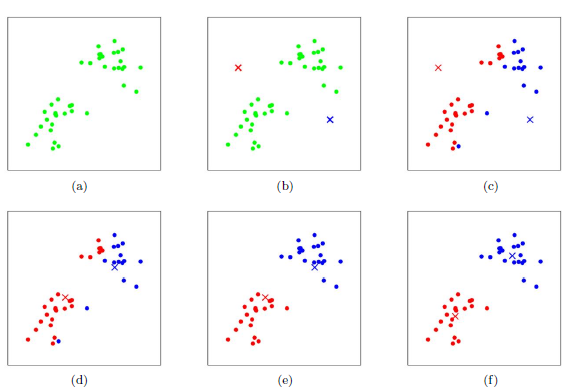
\includegraphics[width=10cm]{cluster4.png}}
	\caption{A concrete $k$-Means clustering process}
	\label{alo:kmeans basic}
\end{figure}

         Shokri, etc. put forward the partial convergence of  the standard $k$-Means algorithm. And they also described how to obtain a local minimum of the $k$-Means clustering problem under certain given conditions with Minkowsky metric. But how to find the global minimum is still a open problem.

         \begin{theorem}[Partial Convergence]
         The standard $k$-Means algorithm converges to a partial optimal solution of $k$-Means clustering problem in a finite number of iterations.
         \end{theorem}

         Here we give no specific proof but the definition of partial optimal solution of $k$-Means clustering problem.
         \begin{definition}
         A point $(W^{*}, c^{*})$ is partial optimal solution of $k$-Means clustering problem if it satisfies the following:
         \begin{equation}
         \phi(W^{*}, c^{*}) \leq \phi(W^{*}, c), \forall c \in \mathbb{R}^{nk};
         \end{equation}
         and
         \begin{equation}
         \phi(W^{*}, c^{*}) \leq \phi(W, c^{*}), \forall W \in M_{k \times N}(R).
         \end{equation}
         \end{definition}

         We give another form of the standard $k$-Means algorithm, which can give proof of theorem \textbf{Partial Convergence}.

	 \begin{algorithm}
		\caption{The Standard $k$-means(another form)}
	         \label{alo:kmeans2}
		\textbf{Input:}  Data set $X=\lbrace x_{1},...,x_{N}| x_{i}\in\mathbb{R}^n\rbrace$ and $k$(and Tol)
		
		\textbf{Output:} The cluster centers $c = ( c^{1},..., c^{k})$
		
		\begin{algorithmic}[1]
		\State Choose the \textbf{initial} centers arbitrarily, $c_{0}=(c_{0}^{1},c_{0}^{2},...,c_{0}^{k})$.
		\State \textbf{Repeat:} for $j \geq 0$
                                  $$
			w_{li}^{j+1} = I(l = \arg\min_{1 \leq l \leq k} ||x_{i}-c_{j}^{l}||_{2}^{2})
				$$
				Update
				$$
			c_{j+1}^{l} = \frac{\sum_{i=1}^{N} w_{li}^{j+1} \cdot x_{i}}{\sum_{i=1}^{N} w_{li}^{j+1} }
				$$
			\textbf{Stop} criterion $$ W^{j+1} = W^{j}$$ or ($||c_{j+1}-c_{j}|| \leq Tol$)
		\State \textbf{Output} $$c = c_{j}$$ 
	   \end{algorithmic}
	   \end{algorithm}

	\subsection{The $k$-Means++ Algorithm}
	The standard $k$-Means algorithm is highly sensitive to the initialization of cluster centers. It is easy to construct situations in which the standard $k$-Means algorithm converges to a local minimum that is arbitrarily bad compared to the optimal solution. Such an example is shown in figure \ref{alo:algorithm ratio} for $k=3$ and where $x<y<z$.

		 \begin{figure}[htbp]
		 	\centering{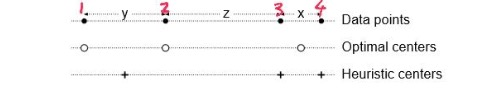
\includegraphics[width=10cm]{algo.png}}
		 	\caption{High approximation ratio}
		 	\label{alo:algorithm ratio}
		 \end{figure}

	       If we initialize cluster centers $(1, 2, 3)$, we can get the optimal centers shown at the middle with the standard $k$-Means algorithm.
	        \begin{equation}
	        \phi^{opt} = (\frac{x}{2})^{2}+(\frac{x}{2})^{2}=(\frac{x^{2}}{2})
	        \end{equation}

	        Unfortunately, if we initialize centers $(2, 3 ,4)$, it is easy to verify that the centers shown at the bottom is the solution, a bad solution.
	         \begin{equation}
	          \phi_{heu} = (\frac{y}{2})^{2}+(\frac{y}{2})^{2}=(\frac{y^{2}}{2})
	        \end{equation}
	        We can see the two different initialization such that the algorithm converges to very different solutions.

	 The following advanced algorithm provides a better initialization of the clustering and gives the $O(\log k)-approximation$ solution.
	 \begin{theorem}
	 \label{competitive}
	 If $\mathcal{C}$ is the cluster result of $k$-Means ++, then the corresponding potential function $\phi$ satisfies that 
	 \begin{equation}
	 E[\phi] \leq 8(\ln k + 2)\phi^{*}
	 \end{equation}
	 \end{theorem}

	The k-means++ algorithm addresses the second of these obstacles above by specifying a procedure to initialize the cluster centers before proceeding with the standard k-means optimization iterations. With the k-means++ initialization, the algorithm is guaranteed to find a solution that is $ O(\log k) $ competitive to the optimal k-means solution. It improves the running time of the standard $k$-Means algorithm (i.e. Lloyd's algorithm), and the quality of the final solution.

	This algorithm is written in Algorithm \ref{alo:kmean++}.

	\begin{algorithm}[H]
		\begin{algorithmic}[1]
			\caption{$k$-Means++}
			\label{alo:kmean++}
			\State $\mathcal{C}\leftarrow$ Choose $c_1$ with a uniform distribution among the data points ($c_1$ is the first center).
			%均匀分布
			\State \textbf{For $l \leq k$},

		Sample $x$ from $X$ with probability $\frac{d^{2}(x, \mathcal{C})}{\phi_{X}(\mathcal{C})}$.
		    
		    $\mathcal{C} \leftarrow \mathcal{C}\cup\{x\}$
		    
		    \State Use the standard $k$-Means algorithm.
		\end{algorithmic}
	\end{algorithm}

         Here we import the definition of probability sampling. These days, we tend to use computers as the mechanism for generating random numbers as the basis for selection. One popular way to pick $x$ in the above algorithm is to:
         \begin{enumerate} [1.]
         \item Random one number $r \in [0, \phi_{X}(\mathcal{C})]$; 
         \item Do subtraction $r = r - d^{2}(x, \mathcal{C})$ until $r \leq 0$;
         \item Choose the above $x$ as the next seed.
         \end{enumerate}
         
         Next we give the proof of theorem \ref{competitive} according to its creator's idea\cite{kmeansplus}.
         
         \begin{lemma}
         \label{corele}
         Let $\mathcal{C}$ be an arbitrary cluster, and $\mathcal{C}^{*}$ be one cluster of the optimal clustering. Choose $u$ centers from $\mathcal{C}^{*} \setminus \mathcal{C}$ and the union of clustering be $X^{u}$. Define $X^{c}$ as $X - X^{u}$. If adding $t \leq u$ randomly centers to $\mathcal{C}$ as the above algorithm \ref{alo:kmean++}'s step $\textbf{1}$ and $\textbf{2}$, let $\tilde{\mathcal{C}}$ denote the result set, and $\tilde{\phi}$ denote the corresponding potential function. Then, 
         \begin{equation}
         E[\phi_{X}(\tilde{\mathcal{C}})] \leq \left(\phi_{X^{c}}(\mathcal{C}) + 8\phi^{opt}_{X^{u}}\right)\cdot (1+H_{t}) + \frac{u-t}{u}\cdot \phi_{X^{u}}(\mathcal{C})         
         \end{equation}
         where 
         \begin{equation}
         H_{t} = \begin{cases}& 1 + \frac{1}{2} + \cdots + \frac{1}{t}, \ \text{$t > 0$}\\
         & 0,\  \text{ $t = 0$}
         \end{cases}
         \end{equation}
         %proof
         \begin{proof}
         
         For convenience, we define probability events as follows.
         \begin{equation}
         \begin{cases}
        & \mathscr{A} = \{\text{add the first center from $X$}\}\\
         & \mathscr{A}_{1} = \{\text{add the first center from $X^{u}$}\}\\
         &\mathscr{A}_{2}= \{\text{add the first center from $X^{c}$}\}\\
         &\mathscr{A}_{1} \cap \mathscr{A}_{2} = \empty, \mathscr{A}_{1} \cup  \mathscr{A }_{2} = \mathscr{A}
         \end{cases}
         \end{equation}
         
         One can split the whole expectation into two branches.
         \begin{equation}
         E[\phi_{X}(\tilde{\mathcal{C}})] = Prob_{\mathscr{A}_{1}} \cdot E[\phi_{X}(\tilde{\mathcal{C}})|\mathscr{A}_{1}] + Prob_{\mathscr{A}_{1}} \cdot E[\phi_{X}(\tilde{\mathcal{C}})|\mathscr{A}_{2}]
         \end{equation}         

         
         Firstly, when $t = 0$ and $u > 0$, i.e. $\phi_{X}(\mathcal{C}^{'}) = \phi_{X}(\mathcal{C})$. it following $1 + H_{t} = 1$ naturally has  
         \begin{equation}
         E[\phi_{X}(\tilde{\mathcal{C}})] \leq \phi_{X^{c}}(\mathcal{C}) + 8\phi^{opt}_{X^{u}} + \phi_{X^{u}}(\mathcal{C})         
         \end{equation}
         
         If $t = u = 1$, there has 
           \begin{equation}
           \label{eqlemma}
           \begin{aligned}
        E[\phi_{X^{u}}(\tilde{\mathcal{C}})|\mathscr{A}_{1}]   = &\sum_{x_{0} \in X^{u}} \frac{d^{2}(x_{0}, \mathcal{C})}{\sum_{x \in X^{u}} d^{2}(x, \mathcal{C})} \sum_{x \in X^{u}} \min \{d^{2}(x, \mathcal{C}), ||x - x_{0}||^{2}\} & \tilde{\mathcal{C}} = \mathcal{C} \cup \{x_{0}\} \\
          \leq &   \sum_{x_{0} \in X^{u}}\frac{ \left(\frac{2}{|X^{u}|} \sum_{x \in X^{u}}  d^{2}(x, \mathcal{C}) + \frac{2}{|X^{u}|} \sum_{x\in X^{u}} ||x - x_{0}||^{2} \right)}{\sum_{x \in X^{u}} d^{2}(x, \mathcal{C})} \cdot & Lemma\  \ref{powermean}\\
         &\sum_{x \in X^{u}} \min \{d^{2}(x, \mathcal{C}), ||x - x_{0}||^{2}\} \\
         \leq &  \frac{4}{|X^{u}|} \sum_{x_{0} \in X^{u}}  \sum_{x\in X^{u}} ||x-x_{0}||^{2} \\
          = & 4\cdot \frac{1}{|X^{u}|}  \sum_{x_{0} \in X^{u}} \left(\sum_{x\in X^{u}} ||x - c^{u}||^{2} + |X^{u}|\cdot ||x_{0} - c^{u}||^{2}\right)& Lemma \ \ref{sum}\\
          = & 8\phi^{opt}_{X^{u}} & Lemma \ref{optle}
         \end{aligned}   
         \end{equation}
         where $c^{u}$ is the true center of $X^{u}$ in optimal cluster.
         Then 
         
         \begin{equation}\begin{aligned}
          E[\phi_{X}(\tilde{\mathcal{C}})] = &\frac{\phi_{X^{u}}(\mathcal{C})}{\phi_{X}(\mathcal{C})} E[\phi_{X}(\tilde{\mathcal{C}})|\mathscr{A}_{1}] + \frac{\phi_{X^{c}}(\mathcal{C})}{\phi_{X}(\mathcal{C})} E[\phi_{X}(\tilde{\mathcal{C}})|\mathscr{A}_{2}]\\     
          \leq &\frac{\phi_{X^{u}}(\mathcal{C})}{\phi_{X}(\mathcal{C})} \left(8\phi^{opt}_{X^{u}} +\phi_{X^{c}}(\mathcal{C}) \right) + \frac{\phi_{X^{c}}(\mathcal{C})}{\phi_{X}(\mathcal{C})} \phi_{X}(\mathcal{C})\\    
          \leq &  2\phi_{X}(\mathcal{C}) + 8\phi^{opt}_{X^{u}}
          \end{aligned}
         \end{equation}
         
          
         %%%%induction
         By using induction method, it is sufficient to suppose that the result holds for the cases that $(t-1, u)$ and $(t-1, u-1)$. With similar analysis method as the case of $t = u =1$, if the event $\mathscr{A}_{2}$ happen with probability, $\frac{\phi_{X^{c}}(\mathcal{C})}{\phi_{X}(\mathcal{C})}$, then we still need choose $t-1$ centers with $u$ being unchanged, i.e., 
         \begin{equation}
         E[\phi_{X}(\tilde{\mathcal{C}})|\mathscr{A}_{2}] \leq \left(\phi_{X^{c}}(\mathcal{C}) + 8\phi^{opt}_{X^{u}}\right)\cdot (1+H_{t-1}) + \frac{u-t + 1}{u}\cdot \phi_{X^{u}}(\mathcal{C})
         \end{equation}
         
         Supposed that $\mathscr{A}_{1}$ happened, more specifically, let the first center be chosen from one clustering set $S \subseteq X^{u}$ and $Prob_{x}$ denote the probability of choosing $x \in S$ as the first center. Besides, we define the event $\mathscr{A}_{1}^{s} = \{\text{add the first center from $S$}\}$ and we have its probability of $\frac{\phi_{S}(\mathcal{C})}{\phi_{X}(\mathcal{C})}$. We can conclude similar conclusion as the equation \ref{eqlemma}.
         $$ \sum_{x \in S} Prob_{x} \cdot \phi_{S}(\mathcal{C}) \leq 8\phi^{opt}_{S} $$ 
         
          \begin{equation}
          \begin{aligned}
         &E[\phi_{X}(\tilde{\mathcal{C}})|\mathscr{A}_{1}^{s}] \\
         = & \sum_{x \in S} Prob_{x} \cdot \left( \left(\phi_{X^{c}}(\mathcal{C}) + \phi_{S}(\mathcal{C})
         + 8\phi^{opt}_{X^{u} - S}\right)\cdot (1+H_{t-1}) + \frac{u-t}{u-1}\cdot \phi_{X^{u}-S}(\mathcal{C})\right)\\
           \leq & \left(\phi_{X^{c}}(\mathcal{C})
         + 8\phi^{opt}_{X^{u} }\right)\cdot (1+H_{t-1}) + \frac{u-t}{u-1}\cdot \phi_{X^{u}-S}(\mathcal{C}) 
           \end{aligned}
         \end{equation}
         
         \begin{equation}
         \begin{aligned}
         &\frac{\phi_{X^{u}}(\mathcal{C})}{\phi_{X}(\mathcal{C})} \cdot E[\phi_{X}(\tilde{\mathcal{C}})|\mathscr{A}_{1}] \\
        = & \sum_{S \subseteq X^{u}} \frac{\phi_{S}(\mathcal{C})}{\phi_{X}(\mathcal{C})} E[\phi_{X}(\tilde{\mathcal{C}})|\mathscr{A}_{1}^{s}]\\ 
         = & \frac{\phi_{X^{u}}(\mathcal{C})}{\phi_{X}(\mathcal{C})} \cdot \left(\phi_{X^{c}}(\mathcal{C}) + 8\phi^{opt}_{X^{u} }\right)\cdot (1+H_{t-1}) + \frac{u-t}{u-1}\cdot \sum_{S \subseteq X^{u}} \frac{\phi_{S}(\mathcal{C})}{\phi_{X}(\mathcal{C})}\cdot \phi_{X^{u} - S}(\mathcal{C})\\
         \leq &  \frac{\phi_{X^{u}}(\mathcal{C})}{\phi_{X}(\mathcal{C})} \cdot \left(\phi_{X^{c}}(\mathcal{C}) + 8\phi^{opt}_{X^{u} }\right)\cdot (1+H_{t-1})  \\
         & + \frac{u-t}{u-1}\cdot \frac{1}{\phi_{X}(\mathcal{C})} \left(\phi_{X^{u}}^{2}(\mathcal{C}) - \frac{1}{u} \cdot \phi_{X^{u}}^{2}(\mathcal{C}) \right) \\
         = & \frac{\phi_{X^{u}}(\mathcal{C})}{\phi_{X}(\mathcal{C})} \cdot \left(\left(\phi_{X^{c}}(\mathcal{C}) + 8\phi^{opt}_{X^{u} }\right)\cdot (1+H_{t-1}) + \frac{u - t}{u} \cdot \phi_{X^{u}}(\mathcal{C}) \right) \\
         \end{aligned}     
         \end{equation}
         
         Then 
         \begin{equation}
         \begin{aligned}
         E[\phi_{X}(\tilde{\mathcal{C}})] = &\frac{\phi_{X^{u}}(\mathcal{C})}{\phi_{X}(\mathcal{C})} E[\phi_{X}(\tilde{\mathcal{C}})|\mathscr{A}_{1}] + \frac{\phi_{X^{c}}(\mathcal{C})}{\phi_{X}(\mathcal{C})} E[\phi_{X}(\tilde{\mathcal{C}})|\mathscr{A}_{2}] \\
         \leq &   \left(\phi_{X^{c}}(\mathcal{C}) + 8\phi^{opt}_{X^{u}}\right)\cdot (1+H_{t-1}) + \frac{u-t }{u}\cdot \phi_{X^{u}}(\mathcal{C}) + \frac{\phi_{X^{c}}(\mathcal{C})}{\phi_{X}(\mathcal{C})} \cdot \frac{\phi_{X^{u}}(\mathcal{C})}{\phi_{X}(\mathcal{C})} \\
         \leq &  \left(\phi_{X^{c}}(\mathcal{C}) + 8\phi^{opt}_{X^{u}}\right)\cdot (1+H_{t-1} + \frac{1}{u}) + \frac{u-t }{u}\cdot \phi_{X^{u}}(\mathcal{C})\\
           \leq &  \left(\phi_{X^{c}}(\mathcal{C}) + 8\phi^{opt}_{X^{u}}\right)\cdot (1+H_{t}) + \frac{u-t }{u}\cdot \phi_{X^{u}}(\mathcal{C})\\
         \end{aligned}     
         \end{equation}
         \end{proof}  
         \end{lemma}
         Considering the cluster $\mathcal{C}$ that just cover the first clustering set $S$ in optimal clustering, after algorithm \ref{alo:kmean++}'s step $\textbf{1}$ and $\textbf{2}$, we get the initial seeding and clustering $\tilde{\mathcal{C}}$, which means applying lemma \ref{corele} with $t = u = k-1$, i.e., we choose $X^{c} = S$, then 
	
	\begin{equation}
	\begin{aligned}
	E[\phi_{X}(\tilde{\mathcal{C}})]  \leq &\sum_{x \in S} Prob_{x} \cdot\left(\phi_{S}(\mathcal{C}) + 8\phi^{opt}_{X} - 8\phi_{S}^{opt}\right)\cdot (1+H_{k-1}) &\text{Lemma \ref{optle}} \\
	\leq &8\phi^{opt}_{X}\cdot (1+\ln k) & H_{k-1} \leq 1+\ln k\\
	\end{aligned}     
	\end{equation}
         
         
         
         
         
         
         \subsection{Scalable $k$-Means++}
         \newcommand{\RNum}[1]{\uppercase\expandafter{\romannumeral #1}}
         $k$-Means$\RNum{2}$ uses an oversampling factor $l = \Omega(k)$, which is inspired by $k$-Means++. As we will see,
         	\begin{algorithm}[H]
		\begin{algorithmic}[1]
			\caption{$k$-Means$\RNum{2}$}
			\label{alo:kmean2}
			\State $\mathcal{C}\leftarrow$ Choose $c_1$ uniformly at random among the data points ($c_1$ is the first center).
			%均匀分布
			\State $\psi \leftarrow \phi_{X}(\mathcal{C})$
			 \State For $O(\log \psi)$ times do 

		$\mathcal{C}^{'} \leftarrow $sample independently $x$ from $X$ with probability $\frac{l \cdot d^{2}(x, \mathcal{C})}{\phi_{X}(\mathcal{C})}$.
		    
		    $\mathcal{C} \leftarrow \mathcal{C}\cup\{x\}$
		    
		    end
		    
		    \State For $x \in \mathcal{C}$, set $\omega_{x}$ to be the number of points in $X$ cluster to $x$ than any other point in $\mathcal{C}$
		    \State Recluster the weighted points in $\mathcal{C}$ into $k$ clusters.
		\end{algorithmic}
	\end{algorithm}
	
          \begin{theorem}
          \label{alo:the}
	 If an $\alpha-approximation$ algorithm is used in Step 5, the Algorithm $\ref{alo:kmean2}$ obtains a solution that is an $O(\alpha)-approximation$ to $k$-Means.
	 \end{theorem}
	 
	 More mathematically, there has 
	  \begin{theorem}
	 Let $\alpha = exp(-(1- e^{-l/(2k)})) \approx e^{-\frac{l}{2k}}$. In Algorithm $\ref{alo:kmeans2}$, 
	 \begin{equation}
	 E[\phi_{X}(\mathcal{C}\cup \mathcal{C}^{'})] \leq 8 \phi^{*} + \frac{1+\alpha}{2} \phi_{X}(\mathcal{C})
	 \end{equation}
	 \end{theorem}
	 
	 \begin{corollary}\label{alo:cor1}
	If $\phi^{(i)}$ is the objective of the clustering after the $i$-th round of Algorithm $\ref{alo:kmeans2}$, then 
	\begin{equation}
	 E[\phi^{(i)}] \leq \frac{16}{1 - \alpha} \phi^{*} + \left(\frac{1+\alpha}{2}\right)^{i} \psi
	 \end{equation}
	 \end{corollary}
	 Corollary $\ref{alo:cor1}$ implies that after $O(\log \psi)$ rounds, the result can touch $O(\phi^{*})$. Then the Theorem is an immediate consequence.
	 
\section{The Choice of $k$}
         In general, we don't know the optimal number of clusters, $k$ in the practical probems. Here we give one method named ``elbow''.
         Elbow method has two step can be written as following:
         \begin{enumerate}
         \item Compute the sum of squared error $(SSE)$ for some values of $l$ (for example $2, 4, 6, 8,$ etc.):
         \begin{equation}
         SSE={\sum_{l=1}^{k}\sum_{x \in S_{l}}} ||x-c_{l}||^{2}
         \end{equation}
         \item Plot $l$ against the SSE, and choose the $k$ at which the $SSE$ decreases abruptly.
\end{enumerate}

         For one example as the figure shown, we will understand how elbow method works.

          \begin{figure}[htbp]
		 	\centering{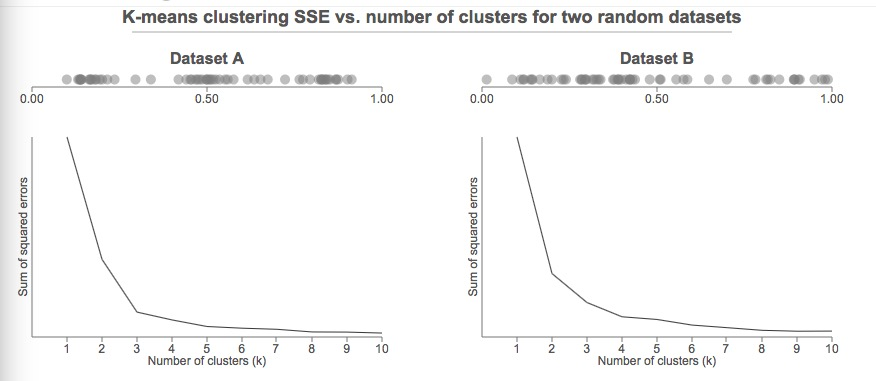
\includegraphics[width=10cm]{cluster_numbers.png}}
		 	\caption{Using the Elbow Method to Determine the Optimal Number of Clusters}
		 \end{figure}

         We note Dataset A on the left. At the top we see a number line plotting each point in the dataset, and below we see an elbow chart showing the SSE after running $k$-Means clustering for $k$ going from $1$ to $10$. We see a pretty clear elbow at $k = 3$, indicating that $3$ is the best number of clusters.

         However, the elbow method doesn't always work well; especially if the data is not very clustered. Notice how the elbow chart for Dataset B does not have a clear elbow. Instead, we see a fairly smooth curve, and it's unclear what is the best value of $k$ to choose.
%%%%%%%%%%%%%%%%%%%%%%%%%%%%%%%%%%%%%%%%%%%%%%%%%%%%%%%%%%%%%%%%%%%%%%%%%%%%%%%%%%%%%%%%%%
\section{Other Contents}
$k$-Means is one type of $k$-Partition clustering, which is about that given a set of $N$ points in Euclidean space and an integer $k$, find a partition of these points into $k$ subsets, each with a center. There are three common formulations of $k$-partition clustering depending on the particular objective used. 
\begin{enumerate}[a.]
\item $k$-Center use the objective to minimize the maximum distance between a point and its nearest cluster center.
\item $k$-Median's objective is to minimize the sum of the distance of each point and its center.
\end{enumerate}
\subsection{Convolutional $k$-Means Clustering}
	Convolutional $k$-Means clustering is another type of algorithms for different problems, because CNN is in general a supervised learning algorithm. We mentioned it here just for complementary.

	Convolutional $k$-Means clustering proposed to train a deep convolutional network based on an enhanced version of the $k$-Means clustering algorithm, which reduces the number of correlated parameters in the form of similar filters, and thus increases test categorization accuracy.

	Generally speaking, this algorithm uses $k$-Means to cluster the parameters of CNN.
